Рассмотрим следующий вызов функции:

\t{label(5, 10, [0, 1, 1, 2], [1, 2, 3, 4])}

В сети находятся $5$ станций, $4$ соединения, соответствующие парам $(0, 1)$, $(1, 2)$, $(1, 3)$ и $(2, 4)$. Каждый из идентификаторов может быть равен числу от $0$ до $k=10$.

Для того, чтобы назначать идентификаторы следующим образом

\begin{center}
\renewcommand{\arraystretch}{1.5}
\begin{tabular}{|c|c|}
\hline
Индекс & Идентификатор  \\
\hline
0 & 6 \\
\hline
1 & 2 \\
\hline
2 & 9 \\
\hline
3 & 3\\
\hline
4 & 7\\
\hline

\end{tabular}
\end{center}

функция \t{label} должна вернуть массив [$6$, $2$, $9$, $3$, $7$]. На рисунке ниже картинка слева демонстрирует индексы вершин, а картинка справа~--- присвоенные идентификаторы.

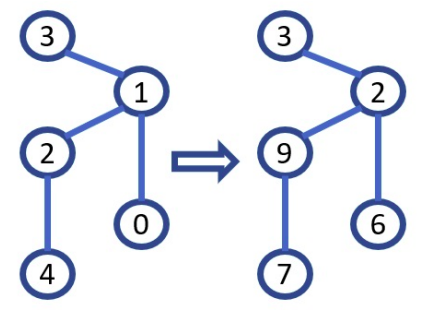
\includegraphics{1.png}

Пусть идентификаторы были присвоены способом, описанным выше. Рассмотрим следующий вызов функции:

\t{find\_next\_station(9, 6, [2, 7])}


Пакет находится на станции с идентификатором $9$, а пункт назначения пакета имеет идентификатор $6$. Идентификаторы станций, лежащих на пути от текущей станции к пункту назначения, равны $[9, 2, 6]$. Таким образом, функция должна вернуть значение $2$, которое соответствует идентификатору станции, куда пакет должен быть передан дальше (эта станция имеет индекс $1$).

Рассмотрим другой возможный вызов функции:


\t{find\_next\_station(2, 3, [3, 6, 9])}

Функция должна вернуть значение $3$, так как пункт назначения, имеющий идентификатор $3$, является соседом станции с идентификатором $2$, а значит, может получить пакет напрямую.

